% Standalone, larger version of Fig. 1 (one gated GRPO training step).
% Not used by main.tex. Compile on its own:  pdflatex fig_training_step.tex  (or tectonic)
% To use it in the paper later: \includegraphics[width=\columnwidth]{figures_standalone/fig_training_step.pdf}
\documentclass[border=6pt]{standalone}
\usepackage{amsmath,amssymb}
\usepackage{tikz}
\usetikzlibrary{positioning,arrows.meta,calc,fit,backgrounds}
\newcommand{\Ahat}{\hat{A}}
\newcommand{\Atil}{\tilde{A}}
\begin{document}
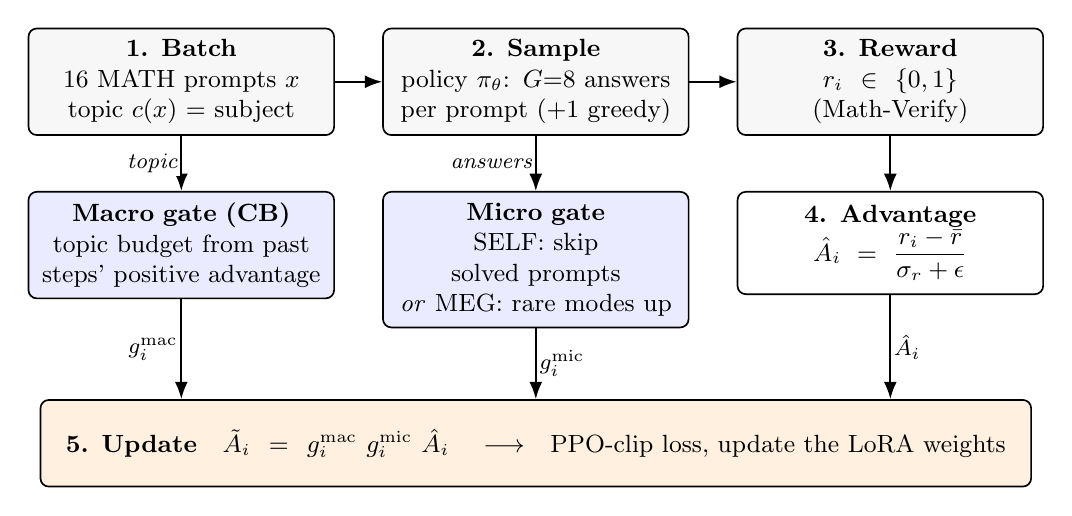
\begin{tikzpicture}[font=\small, node distance=7mm and 6mm,
  box/.style={draw, rounded corners=3pt, align=center, inner sep=4pt, text width=3.6cm, minimum height=13mm,
              line width=0.6pt},
  gate/.style={box, fill=blue!8},
  data/.style={box, fill=gray!6},
  upbox/.style={box, fill=orange!12, text width=12.3cm, minimum height=11mm},
  arr/.style={-{Latex[length=2.2mm]}, line width=0.7pt},
  lab/.style={font=\footnotesize\itshape, fill=white, inner sep=1pt}]

% row 1: data flow of one step
\node[data] (x) {\textbf{1. Batch}\\ 16 MATH prompts $x$\\ topic $c(x)$ = subject};
\node[data, right=of x] (pi) {\textbf{2. Sample}\\ policy $\pi_\theta$: $G{=}8$ answers\\ per prompt (+1 greedy)};
\node[data, right=of pi] (r) {\textbf{3. Reward}\\ $r_i\in\{0,1\}$\\ (Math-Verify)};

% row 2: the two gates and the advantage
\node[gate, below=of x] (mac) {\textbf{Macro gate (CB)}\\ topic budget from past\\ steps' positive advantage};
\node[gate, below=of pi] (mic) {\textbf{Micro gate}\\ SELF: skip solved prompts\\ \emph{or} MEG: rare modes up};
\node[box, below=of r] (adv) {\textbf{4. Advantage}\\ $\Ahat_i = \dfrac{r_i-\bar r}{\sigma_r+\epsilon}$};

% row 3: the update
\node[upbox, below=9mm of mic] (upd)
  {\textbf{5. Update}\quad $\Atil_i \;=\; g^{\mathrm{mac}}_i\; g^{\mathrm{mic}}_i\;\Ahat_i$
   \quad$\longrightarrow$\quad PPO-clip loss, update the LoRA weights};

% arrows
\draw[arr] (x) -- (pi);
\draw[arr] (pi) -- (r);
\draw[arr] (r) -- (adv);
\draw[arr] (x) -- node[lab, left] {topic} (mac);
\draw[arr] (pi) -- node[lab, left] {answers} (mic);
\draw[arr] (adv) -- node[lab, right] {$\Ahat_i$} (adv |- upd.north);
\draw[arr] (mac) -- node[lab, left] {$g^{\mathrm{mac}}_i$} (mac |- upd.north);
\draw[arr] (mic) -- node[lab, right] {$g^{\mathrm{mic}}_i$} (upd);
\end{tikzpicture}
\end{document}
